% Options for packages loaded elsewhere
\PassOptionsToPackage{unicode}{hyperref}
\PassOptionsToPackage{hyphens}{url}
\PassOptionsToPackage{dvipsnames,svgnames,x11names}{xcolor}
\documentclass[
  10pt,
  fontset=fandol]{ctexart}
\usepackage{xcolor}
\usepackage[margin=16mm]{geometry}
\usepackage{amsmath,amssymb}
\setcounter{secnumdepth}{-\maxdimen} % remove section numbering
\usepackage{iftex}
\ifPDFTeX
  \usepackage[T1]{fontenc}
  \usepackage[utf8]{inputenc}
  \usepackage{textcomp} % provide euro and other symbols
\else % if luatex or xetex
  \usepackage{unicode-math} % this also loads fontspec
  \defaultfontfeatures{Scale=MatchLowercase}
  \defaultfontfeatures[\rmfamily]{Ligatures=TeX,Scale=1}
\fi
\usepackage{lmodern}
\ifPDFTeX\else
  % xetex/luatex font selection
\fi
% Use upquote if available, for straight quotes in verbatim environments
\IfFileExists{upquote.sty}{\usepackage{upquote}}{}
\IfFileExists{microtype.sty}{% use microtype if available
  \usepackage[]{microtype}
  \UseMicrotypeSet[protrusion]{basicmath} % disable protrusion for tt fonts
}{}
\makeatletter
\@ifundefined{KOMAClassName}{% if non-KOMA class
  \IfFileExists{parskip.sty}{%
    \usepackage{parskip}
  }{% else
    \setlength{\parindent}{0pt}
    \setlength{\parskip}{6pt plus 2pt minus 1pt}}
}{% if KOMA class
  \KOMAoptions{parskip=half}}
\makeatother
\usepackage{graphicx}
\makeatletter
\newsavebox\pandoc@box
\newcommand*\pandocbounded[1]{% scales image to fit in text height/width
  \sbox\pandoc@box{#1}%
  \Gscale@div\@tempa{\textheight}{\dimexpr\ht\pandoc@box+\dp\pandoc@box\relax}%
  \Gscale@div\@tempb{\linewidth}{\wd\pandoc@box}%
  \ifdim\@tempb\p@<\@tempa\p@\let\@tempa\@tempb\fi% select the smaller of both
  \ifdim\@tempa\p@<\p@\scalebox{\@tempa}{\usebox\pandoc@box}%
  \else\usebox{\pandoc@box}%
  \fi%
}
% Set default figure placement to htbp
\def\fps@figure{htbp}
\makeatother
\setlength{\emergencystretch}{3em} % prevent overfull lines
\providecommand{\tightlist}{%
  \setlength{\itemsep}{0pt}\setlength{\parskip}{0pt}}
\usepackage{amsmath,amssymb,mathtools,needspace}
\xeCJKDeclareCharClass{CJK}{"2032,"0400->"04FF,"2160->"216B,"2460->"2473,"25A0,"25C7,"25CB,"25CF}
\IfFontExistsTF{Arial Unicode MS}{\xeCJKsetup{AutoFallBack=true}\setCJKfallbackfamilyfont{\CJKrmdefault}{Arial Unicode MS}}{}
\setcounter{secnumdepth}{0}
\setlength{\emergencystretch}{2em}
\allowdisplaybreaks
\usepackage{bookmark}
\IfFileExists{xurl.sty}{\usepackage{xurl}}{} % add URL line breaks if available
\urlstyle{same}
\hypersetup{
  pdftitle={引言},
  colorlinks=true,
  linkcolor={Maroon},
  filecolor={Maroon},
  citecolor={Blue},
  urlcolor={Blue},
  pdfcreator={LaTeX via pandoc}}

\title{引言}
\author{}
\date{}

\begin{document}
\maketitle

\subsection{4.1 引言}\label{ux5f15ux8a00}

\subsubsection{4.1.1 数值求积的基本思想}\label{ux6570ux503cux6c42ux79efux7684ux57faux672cux601dux60f3}

有很多实际问题常常需要计算积分才能求解。有些数值方法，如微分方程和积分方程的求解，也都和积分计算有联系。

依据人们所熟知的微积分基本定理，对于积分 \(I=\int_a^b f(x)\,\mathrm{d}x\)，只要找到被积函数 \(f(x)\) 的原函数 \(F(x)\)，便有下列 Newton-Leibniz 公式：

\[
\int_a^b f(x)\,\mathrm{d}x=F(b)-F(a).
\]

但实际使用这种求积方法往往有困难，因为大量的被积函数，诸如 \(\dfrac{\sin x}{x}\)，\(\sin x^2\) 等等，找不到用初等函数表示的原函数；另外，当 \(f(x)\) 是由测量或数值计算给出的一张数据表时，Newton-Leibniz 公式也不能直接运用。因此有必要研究积分的数值计算问题。

积分中值定理告诉我们，在积分区间 \((a,b)\) 内存在一点 \(\xi\)，有下式成立：

\[
\int_a^b f(x)\,\mathrm{d}x=(b-a)f(\xi).
\]

就是说，底为 \(b-a\) 而高为 \(f(\xi)\) 的矩形面积恰等于所求曲边梯形的面积 \(I\)（见图 4.1）。问题在于点 \(\xi\) 的具体位置一般是不知道的，因而难以准确算出 \(f(\xi)\) 的值。我们将 \(f(\xi)\) 称为区间 \([a,b]\) 上的平均高度。这样，只要对平均高度 \(f(\xi)\) 提供一种算法，相应地便获得一种数值求积方法。

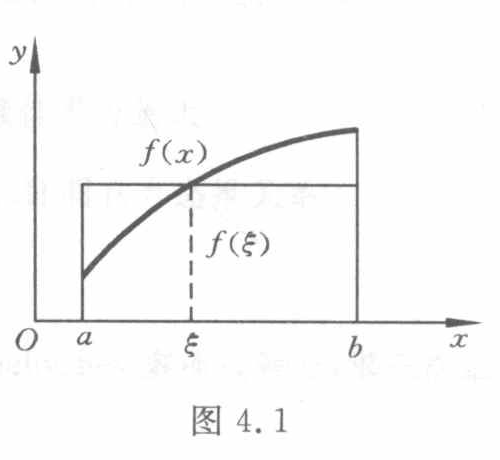
\includegraphics[width=0.85\linewidth,height=\textheight,keepaspectratio,alt={图 4.1（原图裁切）}]{../assets/ch04a/fig-4-1.png}

图 4.1（原图）。图意说明（agent 补充）：曲线 \(f(x)\) 下方从 \(a\) 到 \(b\) 的曲边梯形，与高为 \(f(\xi)\) 的矩形面积相等。图中符号标签：\(x\)，\(y\)，\(O\)，\(a\)，\(\xi\)，\(b\)，\(f(x)\)，\(f(\xi)\)。

如果用两端点的``高度'' \(f(a)\) 与 \(f(b)\) 取算术平均作为平均高度 \(f(\xi)\) 的近似值，这样导出的求积公式

\[
T=\frac{b-a}{2}[f(a)+f(b)]
\tag{4.1.1}
\]

便是我们所熟悉的梯形公式（几何意义参见图 4.2）。如果改用区间中点 \(c=\dfrac{a+b}{2}\) 的

\href{../../source-images/pdf-094.jpeg}{原页图像}

``高度'' \(f(c)\) 近似地取代平均高度 \(f(\xi)\)，则又可导出所谓中矩形公式（以下简称矩形公式）

\[
R=(b-a)f\left(\frac{a+b}{2}\right).
\tag{4.1.2}
\]

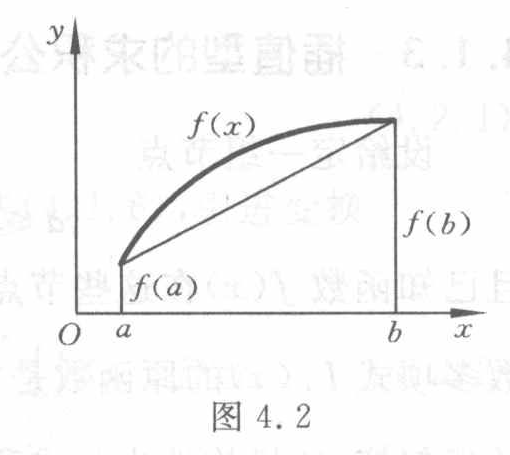
\includegraphics[width=0.85\linewidth,height=\textheight,keepaspectratio,alt={图 4.2（原图裁切）}]{../assets/ch04a/fig-4-2.png}

图 4.2（原图）。图意说明（agent 补充）：用连接曲线 \(f(x)\) 在 \(a\)、\(b\) 两端点的线段形成的梯形近似曲边梯形。图中符号标签：\(x\)，\(y\)，\(O\)，\(a\)，\(b\)，\(f(x)\)，\(f(a)\)，\(f(b)\)。

更一般地，可以在区间 \([a,b]\) 上适当选取某些节点 \(x_k\)，然后用 \(f(x_k)\) 加权平均得到平均高度 \(f(\xi)\) 的近似值，这样构造出的求积公式具有下列形式：

\[
\int_a^b f(x)\,\mathrm{d}x\approx\sum_{k=0}^n A_k f(x_k).
\tag{4.1.3}
\]

其中 \(x_k\) 称为求积节点；\(A_k\) 称为求积系数，亦称伴随节点 \(x_k\) 的权。权 \(A_k\) 仅仅与节点 \(x_k\) 的选取有关，而不依赖于被积函数 \(f(x)\) 的具体形式。

这类数值积分方法通常称为机械求积，其特点是将积分求值问题归结为函数值的计算，这就避开了 Newton-Leibniz 公式需要寻求原函数的困难。

\subsubsection{4.1.2 代数精度的概念}\label{ux4ee3ux6570ux7cbeux5ea6ux7684ux6982ux5ff5}

数值求积方法是近似方法，为保证精度，自然希望求积公式对于``尽可能多''的函数都能准确地成立，这就提出了所谓代数精度的概念。

\textbf{定义 4.1} 如果某个求积公式对于次数不大于 \(m\) 的多项式均能准确地成立，但对于 \(m+1\) 次多项式就不一定准确，则称该求积公式具有 \(m\) 次代数精度。

不难验证，梯形公式（4.1.1）和矩形公式（4.1.2）均具有一次代数精度。

一般地，欲使求积公式（4.1.3）具有 \(m\) 次代数精度，只要令它对于 \(f(x)=1,x,x^2,\cdots,x^m\) 都能准确地成立，这就要求

\[
\begin{cases}
\displaystyle\sum A_k=b-a,\\[4pt]
\displaystyle\sum A_kx_k=\frac12(b^2-a^2),\\
\qquad\vdots\\
\displaystyle\sum A_kx_k^m=\frac{1}{m+1}(b^{m+1}-a^{m+1}).
\end{cases}
\tag{4.1.4}
\]

为简洁起见，这里省略了符号 \(\displaystyle\sum_{k=0}^n\) 中的上、下限。

如果事先选定求积节点 \(x_k\)，譬如，以区间 \([a,b]\) 的等距分点作为节点，这时取 \(m=n\) 求解方程组（4.1.4）即可确定求积系数 \(A_k\)，而使求积公式（4.1.3）至少具有 \(n\) 次代数精度。4.2 节将介绍这样一类求积公式，梯形公式作为其中的一个特例。

构造出形如式（4.1.3）的求积公式的问题，原则上是个确定参数 \(x_k\) 和 \(A_k\) 的代数问题。

\href{../../source-images/pdf-095.jpeg}{原页图像}

\subsubsection{4.1.3 插值型的求积公式}\label{ux63d2ux503cux578bux7684ux6c42ux79efux516cux5f0f}

设给定一组节点

\[
a\leq x_0<x_1<x_2<\cdots<x_n\leq b
\]

且已知函数 \(f(x)\) 在这些节点上的值，作插值函数 \(L_n(x)\)（参见式（2.2.11））。由于代数多项式 \(L_n(x)\) 的原函数是容易求出的，取 \(I_n=\int_a^b L_n(x)\,\mathrm{d}x\) 作为积分 \(I=\int_a^b f(x)\,\mathrm{d}x\) 的近似值，这样构造出的求积公式

\[
I_n=\sum_{k=0}^n A_kf(x_k)
\tag{4.1.5}
\]

是插值型的，其中求积系数 \(A_k\) 通过插值基函数 \(l_k(x)\) 积分

\[
A_k=\int_a^b l_k(x)\,\mathrm{d}x
\tag{4.1.6}
\]

得出。

由插值余项定理（定理 2.2）即知，对于插值型的求积公式（4.1.5），其余项

\[
R[f]=I-I_n=\int_a^b\frac{f^{n+1}(\xi)}{(n+1)!}w(x)\,\mathrm{d}x,
\tag{4.1.7}
\]

其中 \(\xi\) 与变量 \(x\) 有关，\(w(x)=(x-x_0)(x-x_1)\cdots(x-x_n)\)。

如果求积公式（4.1.5）是插值型的，按式（4.1.7），对于次数不大于 \(n\) 的多项式 \(f(x)\)，其余项 \(R[f]\) 等于零，因而这时求积公式至少具有 \(n\) 次代数精度。

反之，如果求积公式（4.1.5）至少具有 \(n\) 次代数精度，则它必定是插值型的。事实上，这时式（4.1.5）对于插值基函数 \(l_k(x)\) 应准确成立，即有

\[
\int_a^b l_k(x)\,\mathrm{d}x=\sum_{j=0}^n A_jl_k(x_j).
\]

注意到 \(l_k(x_j)=\delta_{kj}\)，上式右端实际上即等于 \(A_k\)，因而式（4.1.6）成立。

综上所述，得到如下结论。

\textbf{定理 4.1} 形如式（4.1.5）的求积公式至少有 \(n\) 次代数精度的充分必要条件是，它是插值型的。

\begin{quote}
校注（agent 补充）：式（4.1.7）原扫描将导数阶数印作 \(f^{n+1}(\xi)\)，未带括号；此处按原式保留。由其引用的插值余项定理及上下文，这里表示 \(n+1\) 阶导数。
\end{quote}

\end{document}
